\section{Configuration of the AskoziaPBX}
\label{sec:configuration}
This paragraph is about the configuration of the AskoziaPBX. There is a complete configuration file in the appendix.
First, the used configfile from Askozia is downloaded because the
user should not have to reconfigure the whole box including all accounts and the dialplan after every test. The target is to deliver
the Askozia box just like it was issued. So, there are three necessary steps which are described in the next chapters.
\begin{figure} [htbp]
\centering
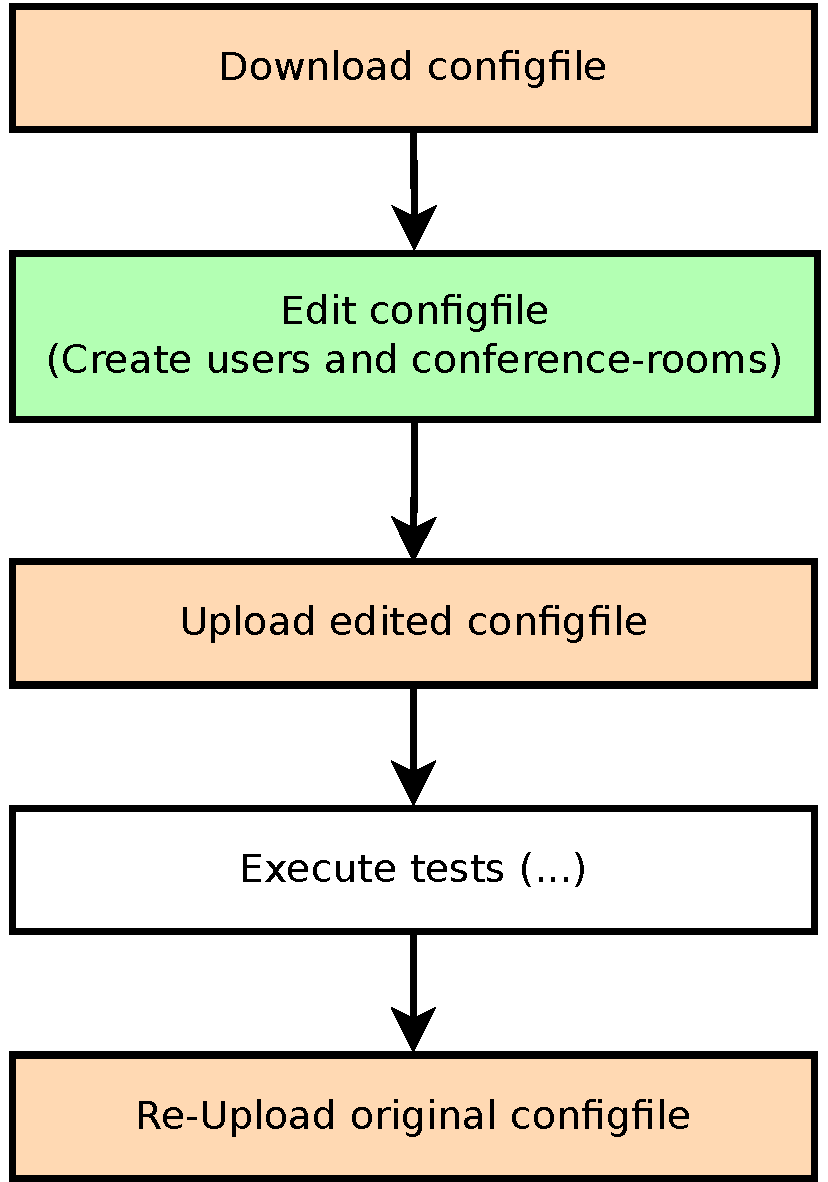
\includegraphics [width=7cm] {config-1}
\caption{Process of editing the Askozia-configfile}
\end{figure}

\subsection{Down-/Upload Configfile}
For downloading the configfile, it is necessary to send a HTML POST request to Askozia. Or, to be more precise, it has to be sent to the qstat-page of the Askozia box. The useragent has to be authenticated as root and the content type must be ``multipart/form-data''. With this POST request, Askozia sends the output of the qstat page. For downloading the configfile, the parameter ``Download'' has to be set to any desired value -- but it has to be set.

In the performance test script, the following perl code is used to send this POST request:
\begin{lstlisting}[breaklines=true,label=code:config-post-request-download,caption={POST request for downloading configfile} ]
use HTTP::Request::Common;
use LWP;
my $ua = new LWP::UserAgent;
$ua->credentials ("$ask_ip:$ask_port",
	$ask_realm, "$ask_user" => "$ask_pw");
my $res = $ua->request (POST
	"http://$ask_ip:$ask_port/$ask_conf_page",
	"Content-Type" => "multipart/form-data",
	Content => [ Download => "1"]);
\end{lstlisting}

After executing this request, the following dataflow has to be expected:
\begin{figure} [h!]
\centering
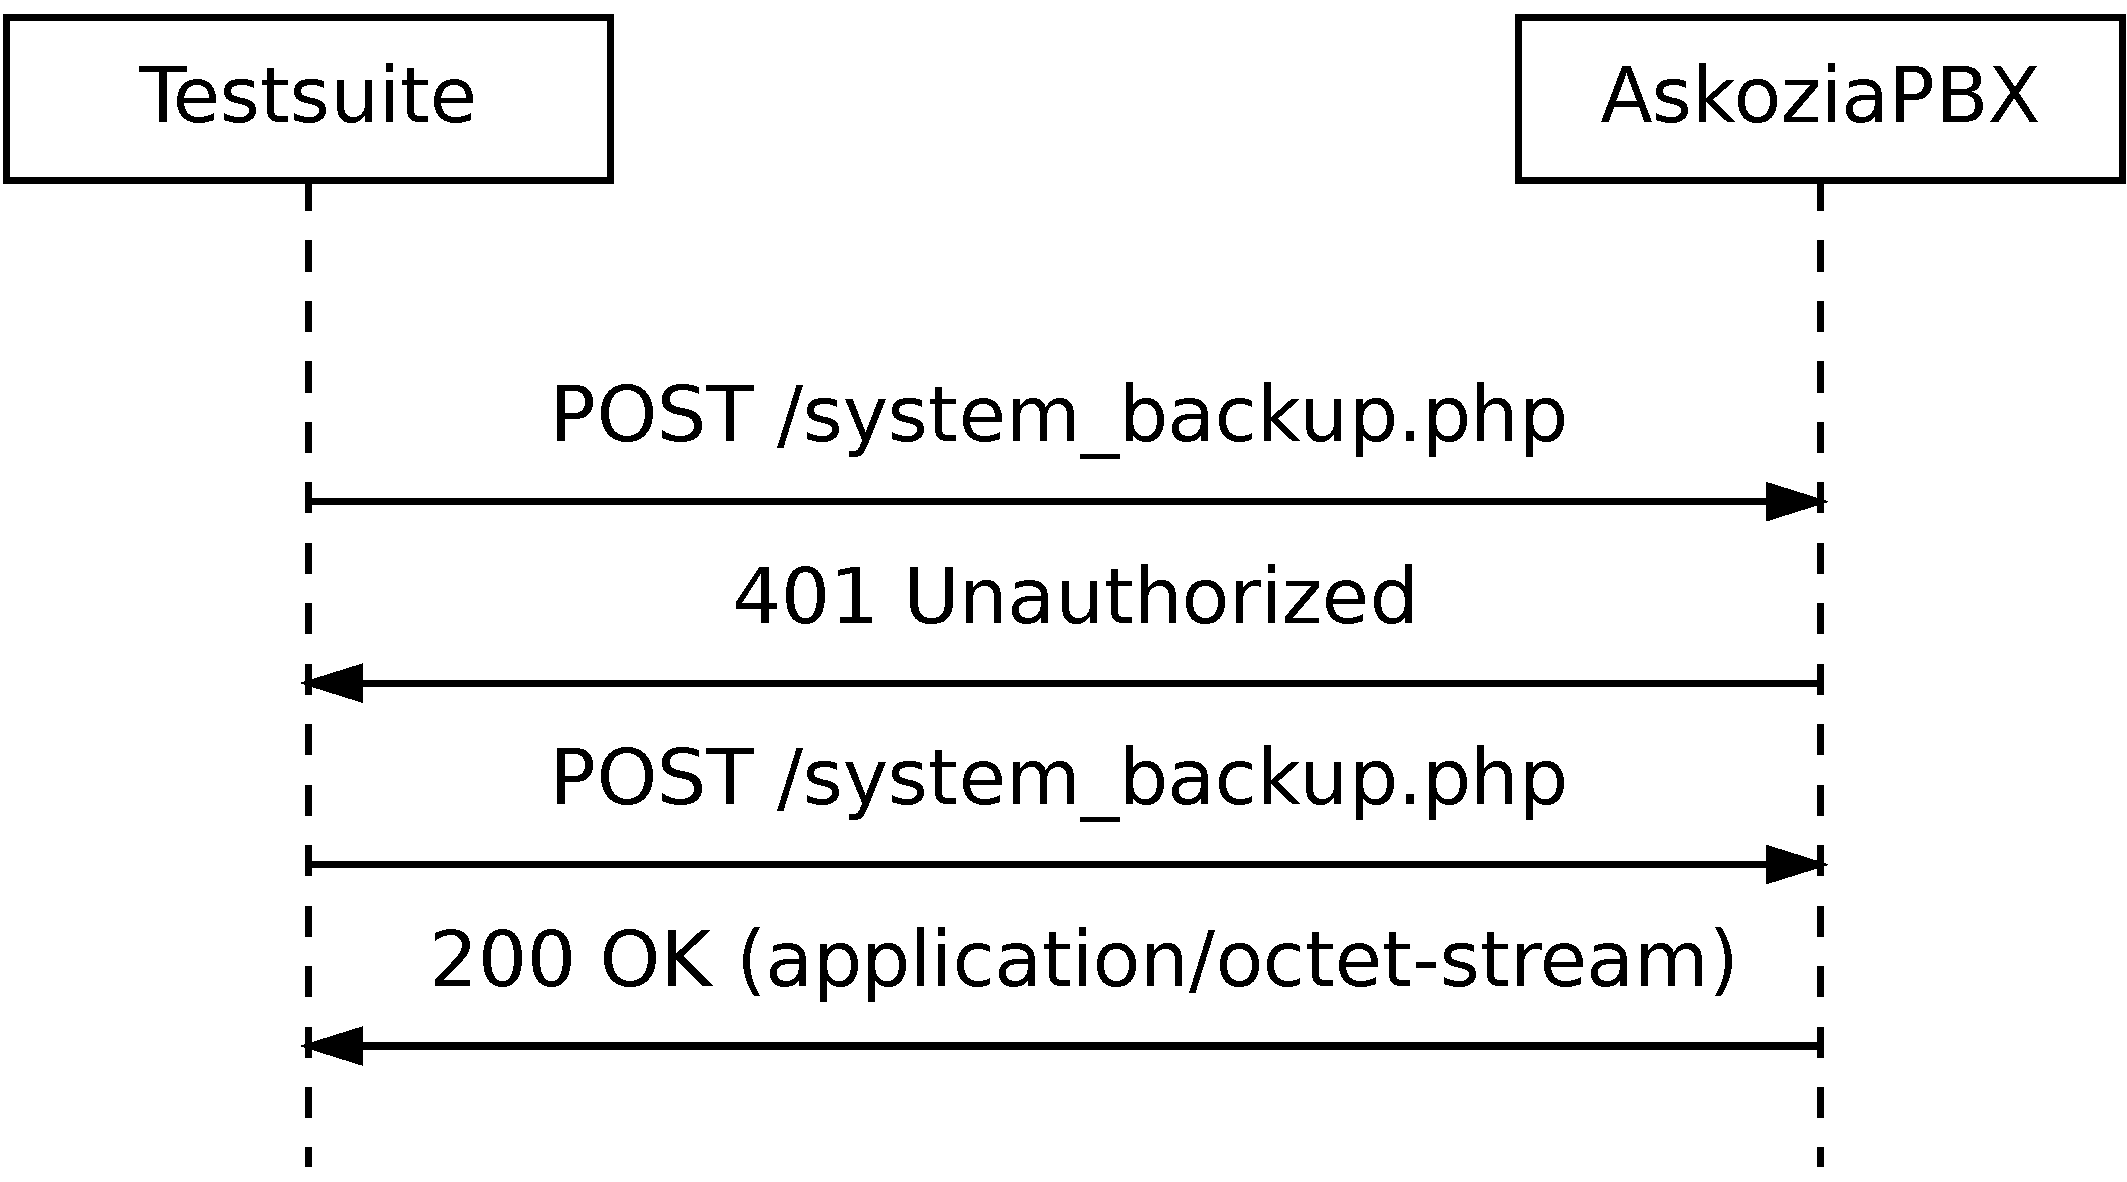
\includegraphics [width=11cm] {config-2}
\caption {Dataflow of configfile download}
\end{figure}

The \texttt{200 OK} message sent by Askozia includes the configfile in xml format. The xml file is saved with its original name
in the \texttt{./results/<testname>/} directory. Then, it is opened for reading to add the needed users and conference rooms
(see the next sections). When finished, the edited configfile is saved with the original named followed by an \texttt{\_edited}
string. This edited configfile is now uploaded to the AskoziaPBX as follows:

\begin{figure} [htbp]
\centering
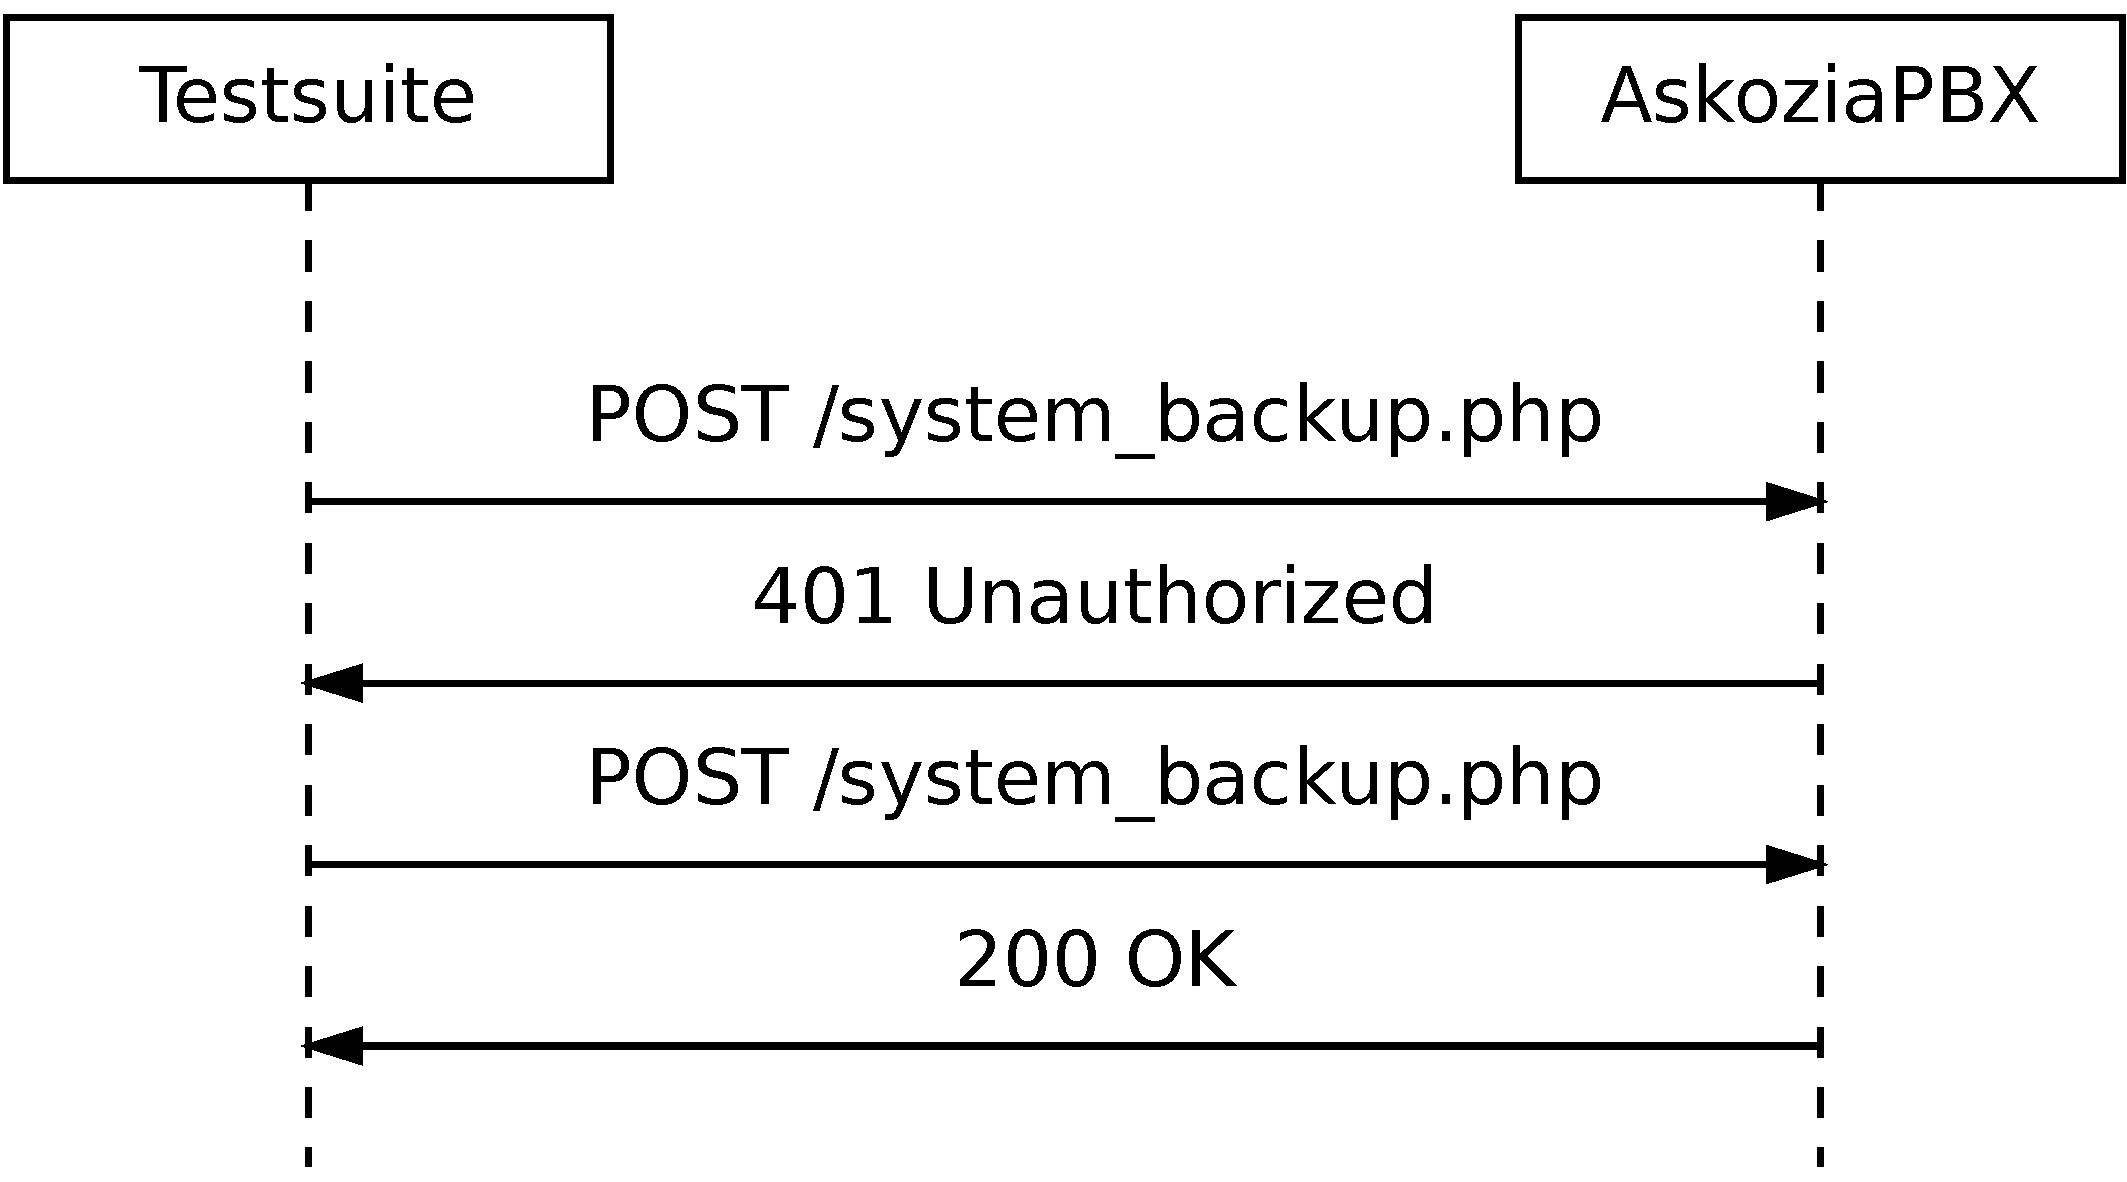
\includegraphics [width=11cm] {config-3}
\caption {Dataflow of configfile upload}
\end{figure}

This dataflow is created by the following perl listing (\texttt{\$ua} and \texttt{\$res} are the existing variables declared and defined above):

\begin{lstlisting}[breaklines=true,label=code:config-post-request-upload,caption={POST request for uploading configfile} ]
$res = $ua->request (POST "http://$ask_ip:$ask_port/$ask_conf_page", "Content-Type" => "multipart/form-data",
    Content => [ Restore => "1", conffile => [ $xml_configfile."_edited" ] ]);
\end{lstlisting}

\subsection{Users}
For executing the planned tests, it is necessary to add some testusers to the AskoziaPBX.
The count of users depends on the parameters that were passed to the script when launching.
Here is a table of needed users, the highest count will be added:

\begin{tabular}{|p{2cm}|p{13cm}|} \hline
	\textsc{Testtype} & \textsc{Needed users} \\ \hline \hline
	two-way & \texttt{= 2 * 2way-calls} (User A and B for each call) \\
	conf room & \texttt{= conf-calls-room * conf-rooms-room} \newline (``conf-calls'' users per ``conf-rooms'' conference rooms) \\
	conf call & \texttt{= conf-calls-call * conf-rooms-call} \newline (``conf-calls'' users per ``conf-rooms'' conference rooms) \\
	\hline
\end{tabular}

The script downloads the complete Askozia configuration file and searches for the begin of the \texttt{sipp} paragraph
Then, it adds its information to the existing phones. It is not checked whether the added phones already exist.
The template for adding users looks as follows, where \texttt{\_userno\_} is replaced by an integer that is incremented with each user:
\begin{lstlisting}[breaklines=true,label=code:config-user-template,caption={User template} ]
<phone>
<extension>User_userno_</extension>
<callerid>Performance-Test Testuser _userno_</callerid>
<codec>ulaw</codec>
<codec>alaw</codec>
<codec>gsm</codec>
<secret>0815</secret>
<uniqid>SIP-PHONE-1357012154bbefaaa79d96_userno_</uniqid>
<language>de-de</language>
<ringlength>indefinitely</ringlength>
<natmode>yes</natmode>
<dtmfmode>auto</dtmfmode>
</phone>
\end{lstlisting}

\subsection{Conference rooms}
Just like the users, the needed conference rooms have to be added, too. So the script searches for the begin of the \texttt{conferencing}
paragraph and adds its needed rooms. The template looks as follows, where \texttt{\_roomno\_} is replaced by an integer that is incremented with each room:
\begin{lstlisting}[breaklines=true,label=code:config-room-template,caption={Conference room template} ]
<room>
<number>_roomno_</number>
<name>Default Conference</name>
<uniqid>CONFERENCE-ROOM-914902610465bd5b50d0c6_roomno_</uniqid>
</room>
\end{lstlisting}

Conference rooms start with number 2663. So, for a conference test that needs ten conference rooms, there are conference rooms 2663 till 2672 created.
